
%%%%%%%%%%%%%%%%%%%%%%%%%%%%%%%%%%%%%%%%%%%%%%%%%%%%%%%%%%%%%%%%%%%%%%%%%
%           Capítulo 2: MARCO TEÓRICO - REVISIÓN DE LITERATURA
%%%%%%%%%%%%%%%%%%%%%%%%%%%%%%%%%%%%%%%%%%%%%%%%%%%%%%%%%%%%%%%%%%%%%%%%%

\chapter{Marco teórico}
Teniendo en cuenta que este proyecto tiene como objetivo la automatización de procesos, empezaremos definiendo conceptos generales relacionados con procesos y automatización, hasta llegar a las definiciones más especificas, se analizarán procesos utilizados dentro del banco que posteriormente se modelarán bajo el estándar Business Process Modeling Notation (BPMN) y se utilizarán las herramientas de Microsoft Power Platform para automatizar dichos procesos.

\section{Dato}
Es una representación simbólica de una variable cualitativa o cuantitativa.

\section{Información}
La información puede definirse como un conjunto de datos procesados y ordenados para su compresión, se lleva a cabo a través de un canal previamente establecido por un emisor y un receptor.
Según Idalberto Chiavenato, información ``es un conjunto de datos con un significado, o sea, que reduce la incertidumbre o que aumenta el conocimiento de algo. En verdad, la información es un mensaje con significado en un determinado contexto, disponible para uso inmediato y que proporciona orientación a las acciones por el hecho de reducir el margen de incertidumbre con respecto a las decisiones'' \citep{chiavenato2019}.

\section{Proceso}
Conjunto de actividades mutuamente relacionadas que utilizan las entradas para proporcionar un resultado previsto \citep{ISO9000}.
\vspace{5mm} %5mm vertical space
\hfill \break
La revista \citep{Revistacatalana1998} define proceso como un conjunto de actividades planificadas que implican la participación de un número de personas y de recursos materiales coordinados para conseguir un objetivo previamente identificado.

\section{Proceso de negocio}
Un ``Proceso de Negocio'' es el flujo o progresión de actividades que se siguen para alcanzar algúnobjetivo del negocio. También se lo define como el conjunto de actividades que sirven para crear valor para el cliente, sea este un cliente externo o interno (otra área del negocio).
Cada proceso tiene un dueño, que es el encargado del proceso. Este “dueño” es el encargado de que el proceso completo se lleve a cabo satisfactoriamente, vinculando tareas para formar un solo trabajo, asegurándose de que el proceso completo funcione bien.\newline
Un ``Proceso de Negocio'' posee las siguientes partes:
\begin{itemize}
	\item Entradas.
		\item Producto o Servicio que genera (Salida).
			\item Recursos que utiliza para generar la salida, ya sean estos humanos o de otro tipo.
\end{itemize}
Además, el proceso de negocio debe estar relacionado con algún objetivo o meta del negocio, y puede incluir otros procesos de Negocio \citep{brunnellomodelado}.
\section{Modelado de procesos}
El modelar los procesos dentro de la organización, permite conocer las áreas problemáticas y susceptibles a mejoras, los niveles y la delegación de
autoridad, las áreas de alto riesgo, el volumen de sus operaciones y el ciclo de vida de sus procesos, incluyendo el contenido tecnológico y la
problemática social.  Una vez que se tiene conocimiento de estos aspectos, los mismos pueden ser utilizados para acelerar o transformar la manera de llevar a cabo el proceso y definir los puntos de interés de la organización sobre los cuales se debe poner más atención \citep{hitpass2017bpm}.
\subsection{Tipos de modelado de procesos}
\begin{itemize}
	\item \textbf{Proceso de negocios interno:} Representa un único proceso de negocio interno donde se representa toda la secuencia del proceso.
	\item \textbf{Proceso de negocios abstracto:} Representa un proceso de negocio externo del que se desconoce los detalles.
	\item \textbf{Proceso de negocio colaborativo:} Representa la interacción entre dos o más entidades del negocio. Las interacciones se representan por los mensajes intercambiados entre las entidades involucradas.
\end{itemize}
\section{Colaborador}
Se hace énfasis en el colaborador como trabajador, y tiene como propósito central que el desempeño de las labores
del trabajador se desarrolle con flexibilidad y autonomía, que exista un reconocimiento por su desempeño, que se posibilite el desarrollo profesional y personal, y que se genere propósito y un sentido con el trabajo que se realiza \citet{Diaz2018}.
\section{Workflow}
Un workflow (flujo de trabajo) en el contexto de las tecnologías de la información, hace referencia a la automatización de un procedimiento de trabajo en el que intervienen documentos, información y tareas que interactúan entre los participantes según un conjunto de reglas definidas, cuyo propósito es alcanzar o contribuir a la consecución de un objetivo de negocio más general. Un flujo de trabajo facilita o automatiza la realización de una parte e la totalidad de un proceso mediante métodos y sistemas informáticos \citep{Hollingsworth1995}.
\section{Automatización}
La automatización es la conversión de un proceso de trabajo, un procedimiento o equipo en automático en lugar
de operación o control humano. La automatización no transfiere simplemente las funciones humanas a las máquinas, sino que
implica una profunda reorganización del proceso de trabajo, durante la cual se redefinen tanto las funciones humanas como las de la máquina \citep{Gerovitch2020}.
\section{Automatización de la Tecnología de Información (TI)}
La automatización de la TI consiste en el uso de sistemas de software para crear instrucciones y procesos repetibles a fin de reemplazar o reducir la interacción humana con los sistemas de TI. El software de automatización funciona dentro de los límites de esas instrucciones, herramientas y marcos, para realizar las tareas con muy poca intervención humana, o sin ella \citep{RedHat2018}.
\section{Automatización empresarial}
La automatización de las empresas consiste en coordinar la gestión de procesos empresariales
(BPM) y la gestión de reglas comerciales (BRM) con el desarrollo de aplicaciones para satisfacer la demanda cambiante del
mercado. Antes, solo bastaba con automatizar los procesos para aumentar la eficiencia y mejorar el control de costos en toda la empresa \citep{RedHat2018}.

\section{BPMN}\label{ch:BPMN}

\subsection{¿Qué es BPMN?}
BPMN es la nomenclatura estándar para el modelado de procesos de negocios. Fue diseñado como una notación de tipo diagrama de flujo robusto, fácil de usar y completamente independiente de la implementación. Los analistas que emplean BPMN no requieren conocer principios de programación orientada a objetos ni algún lenguaje de programación concreto para describir sus procesos de negocio, lo que lo hace ideal para quienes no están relacionados a la industria del software, aunque tampoco excluye a los desarrolladores IT. Su nomenclatura remite a conceptos propios de la programación: intercambio de mensajes, condicionales, ciclos, manejo de excepciones, flujos en paralelo, estados y eventos \citep{lopez2013bpmn}.

\subsection{Eventos}
Un evento es algo que ``sucede'' durante el curso de un proceso. Estos eventos afectan al flujo del modelo y suelen tener una causa (desencadenante) o un impacto (resultado). Los eventos son círculos con centros abiertos para permitir que los marcadores internos diferencien los diferentes disparadores o resultados. Hay tres tipos de eventos, basados en el momento en que afectan al flujo: Inicio, Intermedio y Final \citep{VonRosing2014}.

Representado por círculos, el estilo del borde (línea única, línea doble, línea gruesa) indica el tipo. Los tres tipos de eventos son:

\begin{itemize}
	\item Evento de Inicio (línea única).
	\item Evento Intermedio (línea fina doble)
	\item Evento de Fin (línea gruesa única)
\end{itemize}

\subsubsection{Eventos de inicio}
Un evento de inicio muestra donde empieza un proceso. Un evento de inicio es un pequeño círculo abierto, con una única línea fina como limite.

\begin{table}[H]
	\centering
	\begin{tabular}{ |p{2cm}|p{9.5cm}|p{1.7cm} |  }
		\hline
		\multicolumn{3}{|c|}{Eventos de inicio} \\
		\hline
		\textbf{Elemento}& \textbf{Descripción}&\textbf{Notación}\\
		
		\hline
		{\small Simple } & {\small No se define ningún disparador. } & \vspace{0.5mm} \hspace{2mm} 
\includegraphics[scale=0.2]{Capitulo2/imagenes/Evento2} \\
		
		\hline
		{\small Temporizador } & {\small El disparador son una fecha y hora específicos, o un intervalo de tiempo regular (por ejemplo, el primer viernes de cada mes a las 8am). } & \vspace{2mm} \hspace{2mm} 
\includegraphics[scale=0.2]{Capitulo2/imagenes/EventoT}\\
		
		\hline
		{\small Mensaje } & {\small El disparador es un mensaje que llega desde otra entidad de negocio o rol (participante). Por ejemplo, un cliente pide una verificación de su cuenta. } & \vspace{1mm} \hspace{2mm} 
\includegraphics[scale=0.2]{Capitulo2/imagenes/EventoM}\\
		
		\hline		
		{\small Señal } & {\small  El disparador es una señal difundida desde otro proceso. Por ejemplo, un proceso difunde un cambio en la tasa de interés, disparando cierta cantidad de procesos a iniciarse como resultado.}  &  \vspace{1mm} \hspace{2mm} 
\includegraphics[scale=0.2]{Capitulo2/imagenes/EventoS}\\ 
		
		\hline
		{\small Condicional } & {\small El disparador es una expresión de condición que debe ser satisfecha para que empiece el proceso. } & \vspace{1mm} \hspace{2mm} \includegraphics[scale=0.2]{Capitulo2/imagenes/Eventoc}\\
		
		\hline
		{\small Múltiple } & {\small Define uno o más disparadores que puede ser cualquier combinación de mensajes, temporizadores, condiciones o señales (cualquiera de los cuales inicia un proceso). } & \vspace{1mm} \hspace{2mm} 
\includegraphics[scale=0.2]{Capitulo2/imagenes/EventoMul}\\
		\hline
		\end{tabular}    
		\caption{Eventos de inicio \citep{stephena2009}}
		\label{tabla:Eventosdeinicio}
\end{table}

\subsubsection{Eventos intermedios}
Un evento intermedio es algo que ocurre durante la ejecución de un proceso, estos eventos afectan el flujo del prceso.

\begin{table}[H]
	\centering
	\begin{tabular}{ |p{2cm}|p{9.5cm}|p{1.7cm}|p{1.7cm}|  }
		\hline
		\multicolumn{4}{|c|}{Eventos intermedios} \\
		\hline
		\textbf{Elemento}& \textbf{Descripción}&\textbf{Envío} & \textbf{Recepción}\\
		
		\hline
		{\small Básico } & {\small No se define ningún disparador.  } & &\vspace{0.5mm} \hspace{2mm} 
\includegraphics[scale=0.2]{Capitulo2/imagenes/BasicoR} \\
		
		\hline
		{\small Temporizador } & {\small El disparador son una fecha y hora específicos, o un intervalo de tiempo regular (por ejemplo, el primer viernes de cada mes a las 8am). } & &\vspace{0.5mm} \hspace{2mm} 
\includegraphics[scale=0.2]{Capitulo2/imagenes/TemporizadorR} \\

		
		\hline
		{\small Mensaje } & {\small El disparador es un mensaje. El mensaje debe ser enviado a otra entidad de negocio en el proceso, o debe ser recibido de una de estas. Estas entidades de negocio (participantes), si se muestran en el diagrama, son representadas por Pools(Participantes). } & \vspace{0.5mm} \hspace{2mm} 
\includegraphics[scale=0.2]{Capitulo2/imagenes/MensajeE} &\vspace{0.5mm} \hspace{2mm} 
\includegraphics[scale=0.2]{Capitulo2/imagenes/MensajeR} \\
		\hline
		
		\hline
		{\small Señal } & {\small El diagrama es una señal que se emite o recibe. } & \vspace{0.5mm} \hspace{2mm} \includegraphics[scale=0.2]{Capitulo2/imagenes/SeñalE} &\vspace{0.5mm} \hspace{2mm} \includegraphics[scale=0.2]{Capitulo2/imagenes/SeñalR} \\

		
		\hline
		{\small Error } & {\small Define un evento que normalmente interrumpirá el Proceso o requerirá corrección. } & &\vspace{0.5mm} \hspace{2mm} 
\includegraphics[scale=0.2]{Capitulo2/imagenes/Error} \\
		\hline
		
		\hline
		{\small Vínculo } & {\small Es utilizado para crear un mecanismo visual ``Go To'', ocultando un flujo de secuencia largo, o para establecer conectores ``off-page'', para imprimir. } & \vspace{0.5mm} \hspace{2mm} 
\includegraphics[scale=0.2]{Capitulo2/imagenes/VinculoR} &\vspace{0.5mm} \hspace{2mm} 
\includegraphics[scale=0.2]{Capitulo2/imagenes/VinculoE} \\
		\hline
	\end{tabular}    
	\caption{Eventos intermedios \citep{stephena2009}}
	\label{tabla:Eventosintermedio}
\end{table}

\subsubsection{Eventos finales}
Un evento final marca cuando un proceso, o más especificamente un ``camino'' dentro de un proceso, finaliza nn evento final es un pequeño círculo abierto con una única línea gruesa marcando su límite.

\begin{table}[H]
	\centering
	\begin{tabular}{ |p{2cm}|p{9.5cm}|p{1.7cm} |  }
		\hline
		\multicolumn{3}{|c|}{Eventos finiales} \\
		\hline
		\textbf{Elemento}& \textbf{Descripción}&\textbf{Notación}\\
		
		\hline
		{\small Simple } & {\small No se define ningún resultado. } & \vspace{0.5mm} \hspace{2mm} 
\includegraphics[scale=0.2]{Capitulo2/imagenes/BasicoF} \\
		
		\hline
		{\small Mensaje } & {\small Comunicación con otra entidad de negocio (participante o proceso). } & \vspace{2mm} \hspace{2mm} 
\includegraphics[scale=0.2]{Capitulo2/imagenes/MensajeF}\\
		
		\hline
		{\small Señal } & {\small El diagrama es una señal que se emite o recibe.. } & \vspace{1mm} \hspace{2mm} \includegraphics[scale=0.2]{Capitulo2/imagenes/SeñarT}\\
		
		\hline		
		{\small Error } & {\small  Un estado final que interrumpirá el proceso de transacción.}  &  \vspace{1mm} \hspace{2mm} 
\includegraphics[scale=0.2]{Capitulo2/imagenes/ErrorF}\\ 
		
		\hline
		{\small Compensación } & {\small Usado además como parte del comportamiento del sub-proceso de transacción, este evento lanza el disparador para deshacer (en caso que la instancia necesite ser deshechada). Puede estar vinculado a una actividad específica, o puede dejarse como un evento general de compensación, caso en el cual se aplica globalmente a esta instancia. } & \vspace{1mm} \hspace{2mm} 
\includegraphics[scale=0.2]{Capitulo2/imagenes/CompensacionF}\\
		
		\hline
		{\small Terminador } & {\small Detiene todas las actividades del proceso, incluso si están en curso otros hilos de ejecución. } & \vspace{1mm} \hspace{2mm} 
\includegraphics[scale=0.2]{Capitulo2/imagenes/EventoTer}\\
		\hline
	\end{tabular}    
	\caption{Eventos de inicio \citep{stephena2009}}
	\label{tabla:Eventosdeinicio}
\end{table}

\subsection{Gateway}
Las compuertas o gateways en BPMN son puntos de decisión que pueden ajustar la ruta de un flujo según ciertas condiciones.
\begin{table}[H]
	\centering
	\begin{tabular}{|p{2cm}|p{9.5cm}|p{1.7cm} |}
		\hline
		\multicolumn{3}{|c|}{Tipos de gateways} \\
		\hline
		\textbf{Elemento}& \textbf{Descripción}&\textbf{Notación}\\
		\hline
		{\small Exclusiva } & {\small En un punto de bifurcación, selecciona exactamente un flujo de secuencia de entre las alternativas existentes. En un punto de convergencia, la compuerta espera a que un flujo incidente complete para activar el flujo saliente.} & \vspace{0.5mm} \hspace{2mm} 
\includegraphics[scale=0.1]{Capitulo2/imagenes/gatewayE} \\
		
		\hline
		{\small Basada en eventos } & {\small Esta compuerta siempre será seguida por eventos o tareas de recepción, y sólo activará un flujo saliente dependiendo del evento que ocurra en primer lugar.} & \vspace{0.5mm} \hspace{2mm} 
\includegraphics[scale=0.1]{Capitulo2/imagenes/gatewayBE} \\
		
		\hline
		{\small Paralela } & {\small En un punto de bifurcación, todos los caminos salientes serán activados simultáneamente. En un punto de convergencia, la compuerta espera a que todos los flujos incidentes completen antes de activar el flujo saliente.} & \vspace{0.5mm} \hspace{2mm} 
\includegraphics[scale=0.1]{Capitulo2/imagenes/gatewayP} \\
		\hline
		
		{\small Inclusiva } & {\small En un punto de bifurcación, al menos un flujo es activado. En un punto de convergencia, espera a todos los flujos que fueron activados para activar al saliente.} & \vspace{0.5mm} \hspace{2mm} 
\includegraphics[scale=0.1]{Capitulo2/imagenes/gatewayI} \\
		\hline

		{\small Compleja } & {\small Comportamiento complejo de convergencia/bifurcación no capturado por el resto de compuertas.} & \vspace{0.5mm} \hspace{2mm} 
\includegraphics[scale=0.1]{Capitulo2/imagenes/gatewayC} \\

		
		\hline
		{\small Exclusiva basada en eventos } & {\small En la ocurrencia de uno de los eventos subsecuentes se crea una nueva instancia del proceso.} & \vspace{0.5mm} \hspace{2mm} 
\includegraphics[scale=0.1]{Capitulo2/imagenes/gatewayEBE} \\
		\hline
		

		{\small Paralela basada en eventos  } & {\small En la ocurrencia de uno de los eventos subsecuentes se crea una nueva instancia del proceso.} & \vspace{0.5mm} \hspace{2.5mm} 
\includegraphics[scale=0.1]{Capitulo2/imagenes/gatewayPBE} \\
		\hline
	\end{tabular}
		\caption{Tipos degateways}
\label{tabla:Tiposdegateways}
\end{table}

\subsection{Actividad}
Una actividad se representa mediante un rectángulo de esquinas redondeadas (Figura ~\ref{fig:Actividad}) y es un término genérico para trabajos que la empresa realiza. Una actividad puede ser atómica o no atómica (compuesta).
Las actividades representan acciones, por tanto, una acción es una actividad. Existen dos tipos, actividades atómicas/simples y actividades compuestas/subprocesos. Las actividades atómicas/simples son aquellas que ya no se pueden desagregar en otras y se utilizan para elaborar diagramas a su nivel más bajo de detalle.\\
Las actividades son la espina dorsal de los procesos, debido a que son las actividades las que transforman el estado de un objeto de negocio para que el proceso puede llegar a producir valor para los clientes. Las actividades se pueden definir como acción sobre un objeto, es decir, una actividad se denomina siempre con un verbo (acción) y un sustantivo(objeto). Por ejemplo ``Revisar solicitud'' \citep{hitpass2017bpm}.
\newline
Los tipos de actividades son: 
\begin{figure}[h]
	\centering
	
\includegraphics[scale=0.2]{Capitulo2/imagenes/Actividad} 
	\caption{Actividad}
	\label{fig:Actividad}
\end{figure}

 Los tipos de actividades son: 

\begin{itemize}
	\item \textbf{Tarea:} Una tarea es una unidad de trabajo, el trabajo a realizar. Cuando aparece con el símbolo (+) indica un subproceso, una actividad que puede ser refinada como se ve en la figura ~\ref{fig:Tarea}.
	\begin{figure}[H]
		\centering
		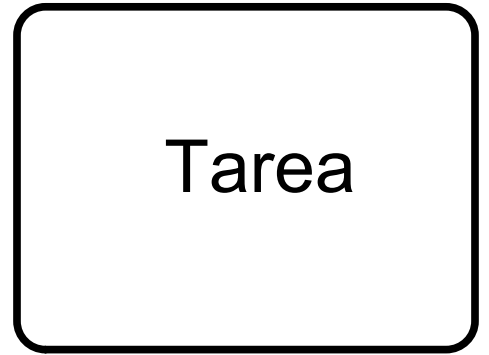
\includegraphics[scale=0.2]{Capitulo2/imagenes/tarea} 
		\caption{Tarea}
		\label{fig:Tarea}
	\end{figure}
	
	\item \textbf{Transacción:} Una Transacción es un conjunto de actividades relacionadas lógicamente, adhiriéndose a un protocolo transaccional particular como se ve en la figura ~\ref{fig:Transaccion}.
	\begin{figure}[h]
		\centering
		
\includegraphics[scale=0.2]{Capitulo2/imagenes/Transaccion} 
		\caption{Transaccion}
		\label{fig:Transaccion}
	\end{figure}
	
	
	\item \textbf{Subproceso de evento:} Un subproceso (figura ~\ref{fig:SubPEvento}) de evento se situa en el interior de otro (sub)proceso. Este se activa en la ocurrencia del evento de inicio especificado y mientras el proceso que lo contiene permanezca también activo. El subproceso de evento puede interrumpir o no al proceso que lo contiene.
	
	\begin{figure}[h]
		\centering
		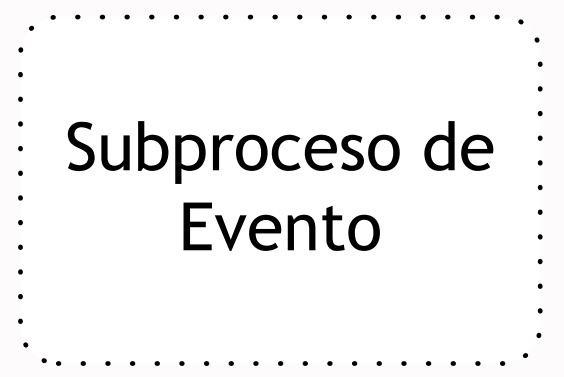
\includegraphics[scale=0.2]{Capitulo2/imagenes/SubPEvento} 
		\caption{Subproceso de evento}
		\label{fig:SubPEvento}
	\end{figure}
	\item \textbf{Actividad de llamada:} Una actividad de llamada es una referencia a un subproceso o tarea definido de forma global que se reutiliza en el proceso actual figura ~\ref{fig:SubPEvento2}.
	\begin{figure}[h]
		\centering
		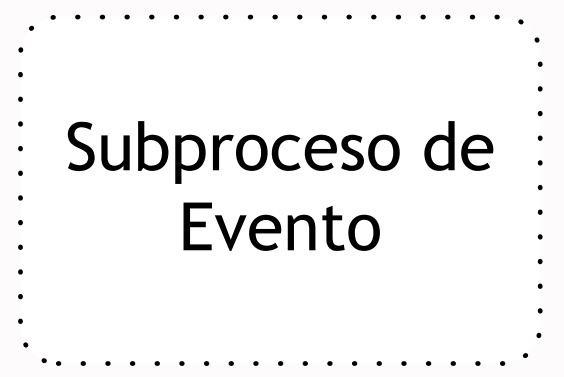
\includegraphics[scale=0.2]{Capitulo2/imagenes/SubPEvento} 
		\caption{Subproceso de evento}
		\label{fig:SubPEvento2}
	\end{figure}
\end{itemize}

\subsubsection{Tarea}
Las tareas son actividades atómicas utilizadas cuando el trabajo que se esta realizando no se puede descomponer a un nivel más detallado. Las tareas son llevadas a cabo por una persona y/o por una aplicación.

\begin{table}[H]
	\centering
	\begin{tabular}{|p{2cm}|p{9.5cm}|p{1.7cm} |}
	\hline
	\multicolumn{3}{|c|}{Tipos de tareas} \\
	\hline
	\textbf{Elemento}& \textbf{Descripción}&\textbf{Notación}\\
	\hline
	{\small Usuario } & {\small Representa el trabajo realizado por un usuario de un sistema conectado al motor de flujo de trabajo. Ejemplo: Registrar un empleado.} & \vspace{0.5mm} \hspace{2mm} 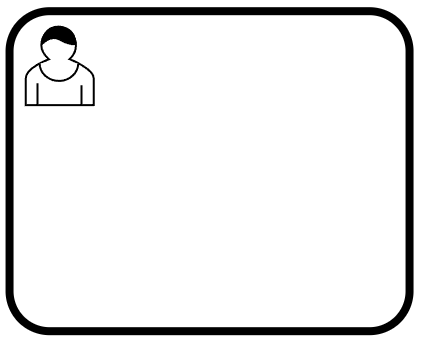
\includegraphics[scale=0.1]{Capitulo2/imagenes/TUsuario} \\
	
	\hline
	{\small Manual } & {\small Representa una tarea realizada por una persona que no utiliza un sistema de workflow. Ejemplo: Servir café.} & \vspace{0.5mm} \hspace{2mm} 
\includegraphics[scale=0.1]{Capitulo2/imagenes/TManual} \\
	
	\hline
	{\small Envío de mensajes } & {\small Envía un mensaje a otro proceso y avanza automáticamente a la siguiente tarea, que normalmente es una tarea de recepción o un evento intermedio de captura de mensajes.} & \vspace{0.5mm} \hspace{2mm} 
\includegraphics[scale=0.1]{Capitulo2/imagenes/TEMensaje} \\
	\hline
	
	{\small Recepción de mensajes } & {\small Espera la recepción de un mensaje desde otro proceso. Normalmente se coloca después de una tarea de envío de mensajes o un evento intermedio de lanzamiento de mensajes.} & \vspace{0.5mm} \hspace{2mm} 
\includegraphics[scale=0.1]{Capitulo2/imagenes/TRMensaje} \\
		
	\hline
	{\small Servicio } & {\small Ejecuta un servicio web y se utiliza para implementar integraciones con sistemas de información.} & \vspace{0.5mm} \hspace{2mm} 
\includegraphics[scale=0.1]{Capitulo2/imagenes/TServicio} \\
		
	\hline
	{\small Regla de negocio } & {\small Acciona una regla de negocio que devuelve un valor para la comparación. Se puede realizar a través de una llamada de servicio web.} & \vspace{0.5mm} \hspace{2mm} 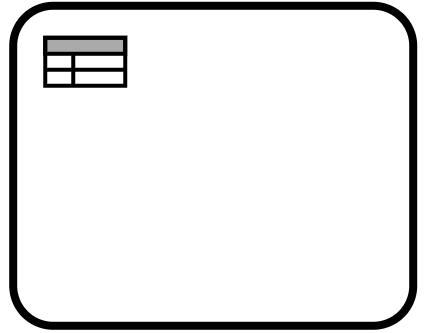
\includegraphics[scale=0.1]{Capitulo2/imagenes/TRNegocio} \\
		\hline
		
	{\small Script } & {\small Ejecuta una secuencia de comandos utilizando el propio motor de procesos. Se puede utilizar, por ejemplo, para ejecutar una secuencia de comandos de Powershell.} & \vspace{0.5mm} \hspace{2mm} 
\includegraphics[scale=0.1]{Capitulo2/imagenes/TScript} \\
		\hline
		
		
	\end{tabular}
	\caption{Tipos de tareas \citep{Bauab2018}}
	\label{tabla:tiposDeTareas}
\end{table}

\subsubsection{Subprocesos}
Un subproceso es un conjunto de actividades incluidas dentro de un
proceso. Puede desglosarse en diferentes niveles de detalle denominadas
tareas. Se representa con un símbolo de suma en la parte central inferior
de la figura. A continuación se presentan los tipos de subprocesos:

\begin{itemize}
	\item \textbf{Colapsada: }Esta versión de Subproceso se ve como una tarea con la adición de un signo más en la parte central inferior (Figura ~\ref{subprocesoC}. Los detalles del sub-proceso no son visibles en el diagrama.
	
	\begin{figure}[H]
		\centering
		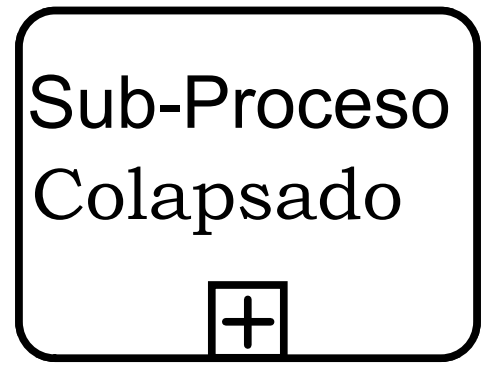
\includegraphics[scale=0.2]{Capitulo2/imagenes/subprocesoC} 
		\caption{Sub-proceso colapsado}
		\label{subprocesoC}
	\end{figure}
	\item \textbf{Expandida: }Esta versión de forma del Sub-proceso es ``estirada'' y abierta para que los detalles de sub-proceso sean visibles dentro de los límites de la forma. en este caso no hay ningún marcador en la parte inferior central de la forma. Sin embargo, algunas herramientas de modelado de procesos colocan un pequeño signo de menos (-) en la parte inferior central de la forma para indicar que el sub-proceso  puede ser colapsado.
\end{itemize}

\subsection{Swimlanes}
Swimlanes ayuda a partir y ordenar las actividades en un diagrama. Hay dos tipos: Pools y Carriles.
\subsubsection{Pool o participantes}
Un Pool es la representación gráfica de un Participante en una Colaboración. Un participante (Figura ~\ref{Pool}) puede ser un PartnerEntity específico (por ejemplo, una empresa) o puede ser un PartnerRole más general (por ejemplo, un comprador, vendedor o fabricante). Un Pool puede o no puede hacer referencia a un proceso. No se requiere que un pool contenga un proceso, es decir, puede ser una “caja negra” \citep{VonRosing2014}.
\begin{figure}[H]
	\centering
	
\includegraphics[scale=0.2]{Capitulo2/imagenes/Pool}
	\caption{Pool o participante}
	\label{Pool}
\end{figure}

\subsubsection{Carriles}
Utilizados a menudo para representar roles de negocio internos dentro de un proceso, los carriles en realidad proveen un mecanismo genérico para particionar los objetos dentro de un pool o participante, basado en las características del proceso o elementos \citep{stephena2009}.
\begin{figure}[H]
	\centering
	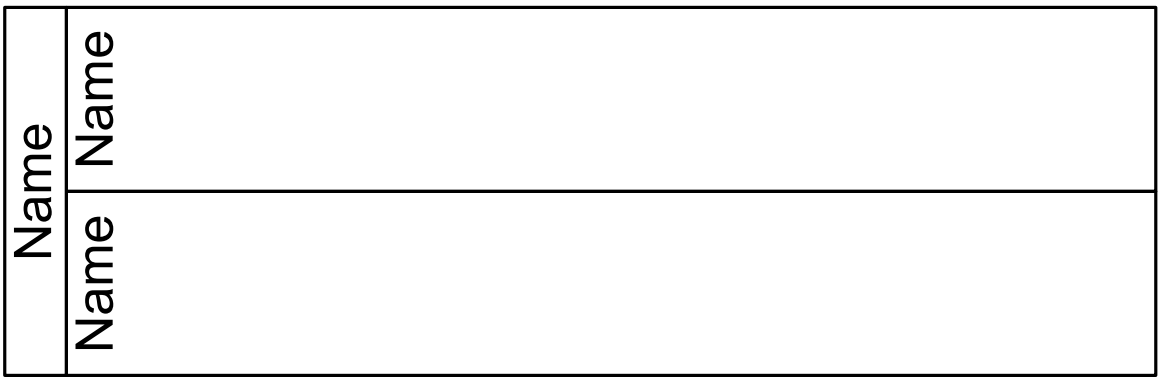
\includegraphics[scale=0.2]{Capitulo2/imagenes/Carril}
	\caption{Carril}
	\label{Carril}
\end{figure}

\subsection{Conectores}
Los conectores vinculan dos objetos en un diagrama. Existen tres diferentes tipos de conectores.

\begin{itemize}
	\item \textbf{Flujo de secuencia: }Define el orden adecuado y conecta los objetos de flujo.
	\begin{figure}[H]
		\centering
		
\includegraphics[scale=0.2]{Capitulo2/imagenes/FlujoDeSecuencia.png}
		\caption{Flujo de secuencia}
		\label{FSecuencia}
	\end{figure}
	\item \textbf{Flujo de mensaje: }Define el flujo de mensajes de un participante de un proceso a otro.
	\begin{figure}[H]
		\centering
		
\includegraphics[scale=0.2]{Capitulo2/imagenes/FlujoDeMensaje.png}
		\caption{Flujo de mensaje}
		\label{FMensaje}
	\end{figure}
	\item \textbf{Asociaciones: }Define las relaciones entre los artefactos y objetos del flujo.
	\begin{figure}[H]
		\centering
		
\includegraphics[scale=0.2]{Capitulo2/imagenes/Asociacion.png}
		\caption{Asociación}
		\label{Asociación}
	\end{figure}
\end{itemize}
\subsection{Artefactos}
Los artefactos proporcionan un mecanismo para capturar información adicional sobre un proceso, más allá de la estructura subyacente de los diagramas de flujo. Esta información no afecta directamente las características del diagrama de flujo de un proceso.

\begin{itemize}
	\item \textbf{Objetos de datos: }Se utiliza para representar los documentos y datos que son manipulados por los procesos. Son como representantes de la ""Carga útil"" del proceso \citep{stephena2009}.
	\begin{figure}[H]
		\centering
		
\includegraphics[scale=0.3]{Capitulo2/imagenes/ObjetoDeDato.png}
		\caption{Objetos de datos}
		\label{Odatos}
	\end{figure}
	
	\item \textbf{Grupos: }Proporciona un mecanismo para resaltar y clasificar una sección del modelo o conjunto de Objetos. \citep{stephena2009}.
	\begin{figure}[H]
		\centering
		
\includegraphics[scale=0.3]{Capitulo2/imagenes/Grupo.png}
		\caption{Grupos}
		\label{Grupos}
	\end{figure}
	
	\item \textbf{Anotaciones de texto: }Añaden más información descriptiva a un modelo.
	\begin{figure}[H]
		\centering
		
\includegraphics[scale=0.3]{Capitulo2/imagenes/Anotacion.png}
		\caption{Anotacion de texto}
		\label{Atexto}
	\end{figure}
	
\end{itemize} 

\section{Herramientas}
\subsection{Power Automate}
Power Automate es una herramienta de flujo de trabajo que permite la automatización de procesos al estilo
evento-a-acción dentro y fuera del conjunto de tecnologías de Microsoft 365. Ofrece conectores externos y la capacidad de
construir conectores externos personalizados hacia y desde otras tecnologías \citet{Critchley2020}.

Power Automate es un servicio de flujo de trabajo en línea que automatiza acciones en las aplicaciones y servicios más comunes. Por ejemplo, puede crear un flujo que agregue un cliente potencial a Microsoft Dynamics 365 y un registro en MailChimp cada vez que alguien con más de 100 seguidores tuitee sobre una empresa.

Cuando se registra, puede conectarse a más de 500 servicios y puede administrar datos en la nube o en fuentes locales como SharePoint y Microsoft SQL Server. La lista de aplicaciones que puede usar con Power Automate crece constantemente \citep{MicrosoftLearn}.

Cuenta con los siguientes tipos de flujos de nube.

\begin{itemize}
	\item \textbf{Flujos automatizados:}	Crear una automatización que se desencadena por un evento como la llegada de un correo electrónico de una persona específica o una mención de la empresa en las redes sociales.
	\item \textbf{Flujos instantáneos:}	Iniciar una automatización con un clic de un botón. Puede automatizar las tareas repetitivas desde el escritorio o dispositivos móviles. Por ejemplo, envíe instantáneamente un recordatorio al equipo con solo presionar un botón desde el dispositivo móvil.
	\item \textbf{Flujos programados:}	Programar una automatización como la carga diaria de datos a SharePoint o una base de datos.
\end{itemize}

\subsection{Power Apps}
Power apps permite a las organizaciones crear e implementar aplicaciones personalizadas que optimizan los
procesos comerciales y mejorar la productividad. Además, Power apps permite a los usuarios crear aplicaciones sin escribir
código, lo que hace posible que los empleados no técnicos obtengan tanto valor de la plataforma como el personal técnico \citep{Pearson2020}.
\subsubsection{Power Apps Studio}
Power Apps Studio es el diseñador de aplicaciones que se usa para compilar aplicaciones de lienzo. El diseñador de aplicaciones hace que la creación de estas se parezca más a la creación de un conjunto de diapositivas en Microsoft PowerPoint \citep{Microsoft}.

\subsection{Power BI}
En pocas palabras, Power BI permite a las organizaciones convertir los datos brutos en información útil que impulsa
una visión empresarial más profunda e informa la toma de decisiones \citet{Pearson2020}.
\subsection{Sharepoint}
Las organizaciones usan Microsoft SharePoint para crear sitios web. Se puede usar como un lugar seguro donde
almacenar, organizar y compartir información desde cualquier dispositivo, así como acceder a ella. Lo que se necesita es un
explorador web, como Microsoft Edge, Internet Explorer, Chrome o Firefox \citet{Microsoft}.

\subsubsection{Listas de Shapoint}
Una lista es una colección de datos que puede compartir con los miembros del equipo y con las personas a las que ha proporcionado acceso. Hay una serie de plantillas de listas base para usar como punto de partida para organizar elementos de lista \citep{Microsoft}.

Las listas de Sharepoint se pueden usar como una base de persistencia de datos o base de datos en dichas listas se puede crear columnas como:

\begin{itemize}
	\item \textbf{Una sola línea de texto: }En este tipo de columnas podemos almacenar cadenas de texto con un límite de hasta 255 caracteres.
	\item \textbf{Varias lineas de texto: }En este tipo de columna podemos almacenar cadenas de texto con más de de 255 carácteres.
	\item \textbf{Número: }En este tipo de columna se puede almacenar datos de tipo numérico no distingue de decimales o enteros, agrupa todos eso tipos de datos en una sola.
	\item \textbf{Sí/No: }En este tipo de columna se puede almacenar valores de sí o no o true o false parecidos a los datos booleanos que se manejan en distintos lenguajes de programación.
	\item \textbf{Usuario: }Este tipo de columna almacena objetos complejos de tipo User, se almacena en un campo datos como el nombre, correo, foto, etc.
	\item \textbf{Fecha y Hora: } En este tipo de columna se puede almacenar valores de tipo fecha parecido a los campos Date que se manejan en distintos lengujes de programación.
	\item \textbf{Opción: }En este tipo de columna se puede almacenar un objeto de valores permitidos, pueden ser varios elemento o solo uno depende del tipo de configuración que se le de.
\end{itemize}

\subsection{Microsoft Forms}
Microsoft Forms es una herramienta para la recolección de datos ya sea por medio de encuestas o
cuestionarios para su posterior manipulación.
\subsection{Power Virtual Agents}
Crea fácilmente chatbots para conversar con los clientes y empleados sin necesidad de escribir
código \citet{Pearson2020}.